\newpage
\section[\textsc{the fundamental theorem of calculus}]{THE FUNDAMENTAL THEOREM OF CALCULUS}\index{Fundamental Theorem of Calculus|(}
The fact that $\dd^2 = 0$ and $\partial^2 = 0$, not to mention the typographical 
similarity of $\dd$ and $\partial$, suggests some connection between chains and forms. 
This connection is established by integrating forms over chains. Henceforth only 
differentiable singular $n$-cubes will be considered.

If $\omega$ ia s $k$-form on $[0,1]^k$, then $\omega = f\dd x^1\wedge\cdots\wedge\dd x^k$
for a unique function $f$. We define 
\begin{align*}
  \int_{[0,1]^k} \omega = \int_{[0,1]^k} f.
\end{align*}

We could also write this as
\begin{align*}
  \int_{[0,1]^k} f\dd x^1\wedge\cdots\wedge\dd x^k = \int_{[0,1]^k} f(x^1,\cdots,x^k)\;\dd x^1\cdots\dd x^k,
\end{align*}

one of the reasons for introducing the functions $x^i$. 

If $\omega$ is a $k$-form on $A$ and $c$ is a singular $k$-cube in $A$, we define
\begin{align*}
  \int_c\omega=\int_{[0,1]^k}c^*\omega.
\end{align*}

Note, in particular, that
\begin{align*}
    \int_{I^k}fdx^1\wedge\cdots\wedge\;\dd x^k
    & = \int\limits_{[0,1]^k}(I^k)^*(f\;\dd x^1\wedge\cdots\wedge \dd x^k) \\
    & = \int_{[0,1]^k}f(x^1,\cdots,x^k)\; \dd x^1\cdots\dd x^k.
\end{align*}

A special definition must be made for $k = 0$. A 0-form $\omega$ is a function; 
if $c:\{0\}\to A$ is a singular 0-cube in $A$ we define
\begin{align*}
  \int_c \omega = \omega(c(0)).
\end{align*}

The integral of $\omega$ over a $k$-chain $c = \sum_{}^{}{a_ic_i}$ is defined by
\begin{align*}
    \int_c\omega=\sum a_i\int_{c_i}\omega.
\end{align*}

The integral\index{Integral!of a form over a chain} of a 1-form over a 1-chain is often called a \textbf{line integral}\index{Line integral}. 
If $P\dd x + Q\dd y$ is a 1-form on $\F{R}^2$ and $c:[0,1]\to\F{R}^2$
is a singular 1-cube (a curve), then one can (but we will not) prove that
\begin{align*}
    \int_c P\dd x+Q\dd y
    & = \lim\sum_{i=1}^n\left[c^1(t_i)-c^1(t_{i-1})\right]\cdot P(c(t^i)) \\
    & \qquad + \left[c^2(t_i)-c^2(t_{i-1})\right]\cdot Q(c(t^i))
\end{align*}
where $t_0,\cdots,t_n$ is a partition of $[0,1]$, the choice of $t^i$ in
$[t_{i-1},t_i]$ is arbitrary, and the limit is taken over all partitions
as the maximum of $|t_i-t_{i-1}|$ goes to 0.The right side is often taken as a definition 
of $\int_c P \dd x + Q \dd y$. This is a natural definition to make, since these sums are 
very much like the sums appearing in the definition of ordinary integrals. However such an 
expression is almost impossible to work with and is quickly equated with an integral equivalent 
to $\int_{[0,1]}c^*(P \dd x+ Q \dd y)$. Analogous definitions for \textbf{surface integrals}\index{Surface integral}\index{Integral!surface}, that
is, integrals of 2-forms over singular 2-cubes, are even more complicated and difficult to use.
This is one reason why we have avoided such an approach. The other reason is that the definition 
given here is the one that makes sense in the more general situations considered in Chapter 5.

The relationship between forms, chains, d, and $\partial$ is summed up in the neatest possible way 
by Stokes' theorem, sometimes called the fundamental theorem of calculus in higher dimensions 
(if $k = 1$ and $c = I^1$ it really is the fundamental theorem of calculus).

\begin{theorem}[Stokes' Theorem]\index{Stokes' Theorem}
    If $\omega$ is a $(k-1 )$-form on an open set $A\subset\F{R}^n$ and $c$ is a $k$-chain in $A$, then
    \begin{align*}
      \int\limits_c\;\dd\omega=\int\limits_{\partial c}\omega.
    \end{align*}
\end{theorem}

\begin{proof}
    Suppose first that $c = I^k$ and $\omega$ is a $(k-1)$-form on $[0,1]^k$.
    Then $\omega$ is the sum of $(k-1)$-forms of the type
    \begin{align*}
      f\dd x^1\wedge\cdots\wedge\widehat{\dd x^i}\wedge\cdots\wedge \dd x^k,
    \end{align*}
    and it suffices to prove the theorem for each of these. This simply involves a 
    computation:

    Note that, if $i=j$, then
    % \begin{align*}
    %     & \int_{[0,1]^{k-1}}I_{(j,{\alpha})}^{*}(f\dd x^1\wedge\cdots\wedge\widehat{dx^i}\wedge\cdots\wedge \dd x^k) \\
    %     & \hspace*{6em} = \left\{\begin{aligned}
    %         & 0 && \text{ if } j\neq i \\
    %         & \int_{[0,1]^k} f(x^1,\cdots,x^k)\;\dd x^1\cdots\dd x^k && \text{ if } j = i
    %     \end{aligned}\right.
    % \end{align*}
    \begin{align*}
      \int_{[0,1]^{k-1}}I_{(j,{\alpha})}^{*}(f\dd x^1\wedge\cdots\wedge\widehat{dx^i}\wedge\cdots\wedge \dd x^k) 
      = \int_{[0,1]^k} f(x^1,\cdots,x^k)\;\dd x^1\cdots\dd x^k
    \end{align*}
    if $i\neq j$, then the left side equals to 0. Therefore 
    \begin{align*}
        & \int_{\partial I^k} f\dd x^1\wedge\cdots\wedge \dd x^k\wedge\cdots\wedge\dd x^k \\
        & = \sum_{j=1}^{k}\sum_{\alpha=0,1}(-1)^{j+\alpha}\int_{[0,1]^{k-1}}I_{(j,\alpha)}^{k}*(f\dd x^1\wedge\cdots\wedge\widehat{\dd x^i}\wedge\cdots\wedge\dd x^k) \\
        & = (-1)^{i+1}\int_{[0,1]^k}f(x^1,\cdots, 1, \cdots,x^k)\dd x^1\cdots \dd x^k \\
        & \hspace*{1em} +(-1)^i\int_{[0,1]^k}f(x^1,\ldots,0,\ldots,x^k)\dd x^1\cdots \dd x^k.
    \end{align*}

    On the other hand,
    \begin{align*}
        & \int_{I^{k}}\;\dd(f \dd x^1\wedge\cdots\wedge\widehat{\dd x^i}\wedge\cdots\wedge \dd x^k) \\
        & = \int_{[0,1]^k}\R{D}_i f\;\dd x^i\wedge\dd x^1\wedge\cdots\wedge\widehat{\dd x^i}\wedge\cdots\wedge\dd x^k \\
        & = (-1)^{i-1}\int_{[0,1]^k} {\R{D}_i f}.
    \end{align*}

    By Fubini's theorem and the fundamental theorem of calculus (in one dimension) we have
    \begin{align*}
        & \int_{I^{k}}\;\dd(f \dd x^1\wedge\cdots\wedge\widehat{\dd x^i}\wedge\cdots\wedge \dd x^k) \\
        & = (-1)^{i-1}\int_{0}^{1}\cdots\left(\int_{0}^{1}\R{D}_{i}f(x^{1},\cdots,x^{k})\;\dd x^{i}\right)\dd x^{1}\cdots\widehat{\dd x^i}\cdots\dd x^k\\
        & = (-1)^{i-1}\int_{0}^{1}\cdots\int_{0}^{1}\big[f(x^{1},\cdots,1,\cdots,x^{k}) \\
        & \hspace*{8.5em} - f(x^{1},\cdots,0,\cdots,x^{k})\big]\;\dd x^{1}\cdots\widehat{\dd x^i}\cdots\dd x^k\\
        & = (-1)^{i-1}\int_{[0,1]^k} f(x^1,\cdots,1,\cdots,x^k)\;\dd x^1\cdots\dd x^k \\
        & + (-1)^{i-1}\int_{[0,1]^k} f(x^1,\cdots,0,\cdots,x^k)\;\dd x^1\cdots\dd x^k.
    \end{align*}

    Thus 
    \begin{align*}
        \int_{I^k}\;\dd\omega=\int_{\partial I^k}\omega.
    \end{align*}

    If $c$ is an arbitrary singular $k$-cube, working through the definitions will show that
    \begin{align*}
        \int_{\partial c}\omega=\int_{\partial I^k}c^*\omega.
    \end{align*}

    Therefore 
    \begin{align*}
        \int_{c}\;\dd\omega
        = \int_{I^{k}}c^{*}(\dd\omega)
        = \int_{I^{k}}\;\dd(c^{*}\omega)
        = \int_{\partial I^{k}}c^{*}\omega
        = \int_{\partial c}\omega.
    \end{align*}

    Finally, if $c$ is a $k$-chain $\sum a_ic_i$, we have 
    \begin{align*}
        \int_c\;\dd\omega
        = \sum a_i\int_{c_i}\;\dd\omega
        = \sum a_i\int_{\partial c_i}\omega
        = \int_{\partial c}\omega.
    \end{align*}
\end{proof}

Stokes' theorem shares three important attributes with
many fully evolved major theorems:
\begin{enumerate}[label=\arabic*.]
    \item It is trivial. 
    \item It is trivial because the terms appearing in it have been properly defined.
    \item It has significant consequences.
\end{enumerate}
Since this entire chapter was little more than a series of definitions which made the 
statement and proof of Stokes' theorem possible, the reader should be willing to grant the
first two of these attributes to Stokes' theorem. The rest of the book is devoted to 
justifying the third.
\index{Fundamental Theorem of Calculus|)}

\begin{problems}
    \problem{ (\textit{Independence of parameterization})\index{Parameterization, independence of}\index{Independence of parameterization}.
        Let $c$ be a singular $k$-cube and $p:[0,1]^k\to [0,1]^k$ a 1-1 function such that 
        $p([0,1]^k) = [0,1]^k$ and $\det p'(x)\ge 0$ for $x\in [0,1]^k$. If $\omega$ is a 
        $k$-form, show that 
        \begin{align*}
            \int_{c}\omega=\int_{c\circ p}\omega.
        \end{align*}
    }
    \problem{
        Show that $\int_{c_{R,n}}\;\dd\theta =2\pi n$, and use Stokes' theorem to conclude
        that $c_{R,n}\neq \partial c$ for any 2-chain $c$ in $\F{R}^2-\{0\}$ (Recall the definition
        of $c_{R,n}$ in Problem 4-23).
    }
    \problem{
        Show that the integer $n$ of Problem 4-24 is unique. This integer is called 
        the \textbf{winding number}\index{Winding number} of $c$ around 0.
    }
    \problem{
        Recall that the set of complex numbers\index{Complex numbers} $\F{C}$ is simply $\F{R}^2$ 
        with $(a,b) = a + b\R{i}$. If $a_1,\cdots,a_n \in \F{C}$ let 
        $f\colon{}\F{C}\to \F{C}$ be $f(z)= z^n + a_1z^{n-1} + \cdots+a_n$. Define singular 
        1-cube $c_{R,f}:[0,1]\to \F{C}-\{0\}$ by $c_{R,f}(t) = f\circ c_{R,1}$, and 
        the singular 2-cube $c$ by $c(s,t) =t\cdot c_{R,n}(s) + (1-t)c_{R,f}(s)$.
        \begin{enumerate}[label=(\alph*)]
            \item Show that $\partial c=\partial c_{R,f} - c_{R,n}$, and that $c([0,1]\times[0,1])\subset
                \F{C}-\{0\}$ if $R$ is large engouh.
            \item Using Problem 4-26, prove the \textit{Fundamental Theorem of Algebra}\index{Fundamental Theorem of Algebra}
              \index{Algebra, Fundamental Theorem of}: 
                Every polynomial $z^n+a_1z^{n-1}+\cdots+a_n$ with $a_i\in\F{C}$ has a root 
                in $\F{C}$.
        \end{enumerate}
    }
    \problem{
        If $\omega$ is a 1-form $f\,\dd x$ on $[0,1]$ with $f(0) = f(1)$, 
        show that there is a unique number $\lambda$ such that $\omega-\lambda \dd x = \dd g$ 
        for some function $g$ with $g(0) = g(1)$. \textit{Hint:} 
        Integrate $\omega-\lambda\dd x = \dd g$ on $[0,1]$ to find $\lambda$.
    }
    \problem{
        If $\omega$ is a 1-form on $\F{R}^2-\{0\}$ such that $\dd\omega = 0$, 
        prove that
        \begin{align*}
            \omega = \lambda\dd\theta + \dd g
        \end{align*}

        for some $\lambda\in\F{R}$ and $g\colon{}\F{R}^2-\{0\}\to\F{R}$. \textit{Hint:} If 
        \begin{align*}
            c_{R,1}^*(\omega) = \lambda_R\dd x + \dd (g_R),
        \end{align*}
        show that all numbers $\lambda_R$ have the same value $\lambda$.
    }
    \problem{
        If $\omega \neq 0$, show that there is a chain $c$ such that 
        $\int_c \omega \neq 0$. Use this fact, Stokes' theorem and $\partial^2 = 0$ 
        to prove $\dd^2 = 0$.
    }
    \problem{
        \begin{enumerate}[label=(\alph*)]
            \item Let $c_1, c_2$ be singular 1-cubes in $\F{R}^2$ with $c_1(0) = c_2(0)$ 
                and $c_1(1)= c_2(1)$. Show that there is a singular 2-cube $c$ such that 
                $\partial c = c_1- c_2 + c_3 - c_4$, where $c_3$ and $c_4$ are degenerate\index{Degenerate singular cube}, 
                that is, $c_3([0,1])$ and $c_4([0,1])$ are points. Conclude that $\int_{c_1}\omega = \int_{c_2}\omega$ 
                if $\omega$ is exact. Give a counterexample on $\F{R}^2-\{0\}$ if $\omega$ is 
                merely closed.
            \item If $\omega$ is a 1-form on a subset of $\F{R}^2$ and $\int_{c_1}\omega = \int_{c_2}\omega$ 
            for all $c_1, c_2$ with $c_1(0) = c_2(0)$ and $c_1(1) = c_2(1)$, show that $\omega$ is exact.
            \textit{Hint:} Consider Problems 2-21 and 3-34.
        \end{enumerate}
    }
    \problem{(\textbf{A first course in complex variables.}\index{Function!differentiable})\index{Complex variables} 
        If $f\colon{} \F{C}\to \F{C}$, define $f$ to be \textbf{differentiable}\index{Differentiable function} at $z_0\in \F{C}$ if 
        the limit
        \begin{align*}
            f'(z_0)=\lim_{z\to z_0}\frac{f(z)-f(z_0)}{z-z_0}
        \end{align*}

        exists.(This quotient involves two complex numbers and this
        definition is completely different from the one in Chapter 2.)
        If $f$ is differentiable at every point $z$ in an open set $A$ and $f'$ is
        continuous on $A$, then $f$ is called \textbf{analytic}\index{Analytic function}\index{Function!analytic} on $A$.
        \begin{enumerate}[label=(\alph*)]
            \item Show that $f(z)=z$ is analytic and $f(z)=\bar{z}$ is not (where $\overline{x-y\R{i}} = x+y\R{i}$).
                    Show that the sum, product, and quotient of analytic functions are analytic. 
            \item If $f=u+v\R{i}$ is analytic on $A$, show that $u$ and $v$ satisfy the \textit{Cauchy-Riemann equations}\index{Cauchy-Riemann equations}:
                \begin{align*}
                    \frac{\partial u}{\partial x} = \frac{\partial v}{\partial y} 
                    && \text{ and } && 
                    \frac{\partial u}{\partial y} = -\frac{\partial v}{\partial x}.
                \end{align*}

                \textit{Hint}:Use the fact that $\lim_{z\to z_0}{[f(z)-f(z_0)]/(z-z_0)}$ must 
                be the same for $z=z_0+(x+\R{i}\cdot 0)$ and $z=z_0+(0+\R{i}\cdot y)$ with 
                $x,y\to 0$. (The converse is also true, if $u$ and $v$ are continuously differentiable;
                this is more difficult to prove.)
            \item Let $T:\F{C}\to \F{C}$ be a linear transformation (where $\F{C}$ is considered 
                as a vector space over $\F{R}$). If the matrix of $T$ with respect to the 
                basis $(1,\R{i})$ is $\begin{pmatrix}a & b\\c & d\end{pmatrix}$ show that
                $T$ is multiplication by a complex number if and only if $a=d$ and $b=-c$. Part (b)
                shows that an analytic function $f\colon{}\F{C}\to\F{C}$, considered as a function $f\colon{}\F{R}^2\to\F{R}^2$,
                has a derivative $\R{D}f(z_0)$ which is multiplication by a complex number. What complex number
                is this ?
            \item Define\index{Lac locus}% what is this 'Lac locus' ???? 
                \begin{align*}
                    \dd(\omega + \R{i}\eta) & = \dd\omega + \R{i}\dd\eta, \\[1em]
                    \int_{c}^{}{\omega + \R{i}\eta} & = \int_{c}^{}\omega + \R{i}\int_{c}^{}\eta, \\[1em]
                    (\omega+\R{i}\eta)\wedge(\theta+\R{i}\lambda)
                        = \omega&\wedge\theta - \eta\wedge\lambda + \R{i}(\eta\wedge\theta + \omega\wedge\lambda),
                \end{align*}
                and 
                \begin{align*}
                    \dd z = \dd x + \R{i}\dd y.
                \end{align*}
                Show that $\dd(f\cdot\dd z)=0$ if and only if $f$ satisfy the Cauchy-Riemann equations.
            \item Prove the \textit{Cauchy Integral Theorem}:\index{Cauchy Integral Theorem}\index{Integral Theorem, Cauchy} If $f$ is analytic on $A$,
                then $\int_c f \dd z = 0$ for every \textbf{closed curve}\index{Curve!closed}\index{Closed curve} $c$ (singular 1-cube with
                $c(0) = c(1)$) such that $c = \partial c'$ for some 2-chain $c'$ in $A$.
            \item Show that if $g(z)=1/z$, then $g\cdot\dd z$ [or $(1/z)\dd z$ in classical notation]
                equals $\R{i}\dd\theta + \dd h$ for some function $h\colon{}\F{C}-\{0\}\to\F{R}$. Concluded
                that $\int_{c_{R,n}}(1/z)\dd z = 2\pi n \R{i}n$.
            \item If $f$ is analytic on $\{z: |z| < 1\}$, use the fact that $g(z)=f(z)/z$ is 
                analytic in $\{z: 0 < |z| < 1\}$ to show that
                \begin{align*}
                    \int_{c_{R_1,n}}\frac{f(z)}z\;\dd z=\intop_{c_{R_2,n}}\frac{f(z)}z\;\dd z
                \end{align*}

                if $0<R_1,R_2<1$. Use (f) to evaluate $\lim\limits_{R\to0}{\int_{C_{R,n}} f(z)/z}\;\dd z$
                and conclude:\par 
                \qquad\textit{Cauchy Integral Formula:}\index{Cauchy Integral Formula}\index{Integral Theorem, Cauchy} If $f$ is analytic on $\{z:|z|<1\}$ and 
                $c$ is a closed curve in $\{z:|z|<1\}$ with winding number $n$ around 0, then
                \begin{align*}
                    n\cdot f(0) = \frac{1}{2\pi\R{i}}\int_{c}\frac{f(z)}{z}\;\dd z.
                \end{align*}
        \end{enumerate}
    }
    \problem{
        If $f\colon{}[0, 1]^2 \to\F{R}^3$ and $s\in [0,1]$ define $F_s:[0,1]\to\F{R}^3$ by 
        $F_s(t)=F(s,t)$. If each $F_s$ is a closed curve, $F$ is called a \textbf{homotopy}\index{Homotopy}
        between the closed curve $F_0$ and the closed curve $F_1$. Suppose $F$ and $G$ are
        homotopies of closed curves; if for each $s$ the closed curves $F_s$ and
        $G_s$ do not intersect, the pair $(F,G)$ is called a homotopy between the
        nonintersecting closed curves $F_0, G_0$ and $F_1, G_1$. It is intuitively
        obvious that there is no such homotopy with $F_0, G_0$ the pair of
        curves shown in Figure \ref{Fig 4-6} (a), and $F_1, G_1$ the pair of (b) or (c).
        The present problem, and Problem 5-33 prove this for (b) but the
        proof for (c) requires different techniques. 
        \begin{enumerate}[label=(\alph*)]
            \item If $f,g\colon{}[0,1]\to\F{R}$ are nonintersecting closed curves define 
                $c_{f,g}:[0,1]^2\to\F{R}^3-\{0\}$ by 
                \begin{align*}
                    c_{f,g}(u,v)=f(u)- g(v).
                \end{align*}

                If $(F,G)$ is a homotopy of nonintersecting closed curves define 
                $C_{F,G}:[0,1]^3\to\F{R}^3-\{0\}$ by 
                \begin{align*}
                    C_{F,G}(s,u,v)=c_{F_s,G_s}(u,v)=F(s,u)-G(s,v).
                \end{align*}

                Show that 
                \begin{align*}
                    \partial C_{F,G}=c_{F_0,G_0}-c_{F_1,G_1}.
                \end{align*}
            \item If $\omega$ is a closed 2-form on $\F{R}^3-\{0\}$ show that 
                \begin{align*}
                  \int_{c_{R_0,G_0}}\omega = \int_{c_{F_1,G_1}}\omega.
                \end{align*}
        \end{enumerate}
    }
\end{problems}
% \clearpage
\begin{figure}[!htb]
    \centering
    \includegraphics[width=.65\linewidth]{./pics/Fig4-6-(a).pdf}
    
    \includegraphics[width=.65\linewidth]{./pics/Fig4-6-(b).pdf}
    
    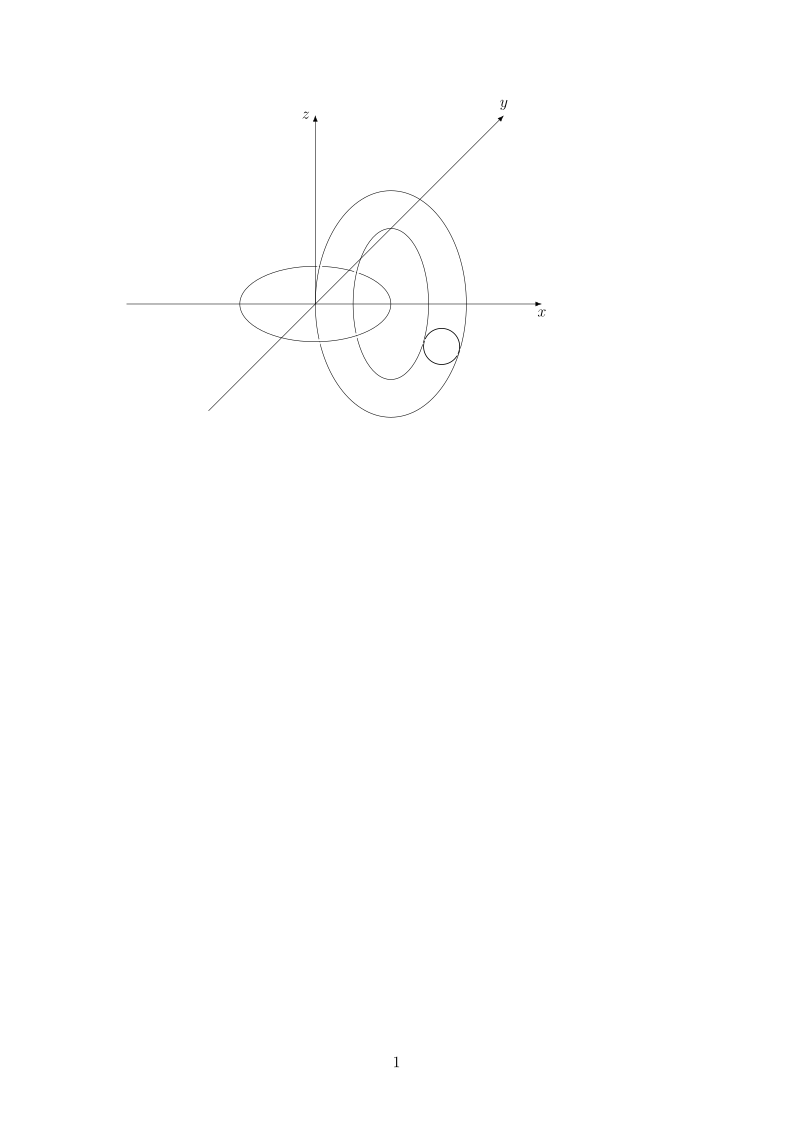
\includegraphics[width=.65\linewidth]{./pics/Fig4-6-(c).pdf}
    \caption{}
    \label{Fig 4-6}
\end{figure}